% ---
% school: "college"
% level: "8eme"
% section: null
% chapter: "التناظر المركزي"
% source: "Axiomaths"
% title: "نقطتان متناظرتان على مستقيمين"
% country: "Tunisie"
% year: 2026
% professor: "Axiomaths"
% difficulty: "Difficile"
% points: null
% tags: ["symetrie-centrale", "construction", "droites", "discussion"]
% ---
% Exercice 13/15 de la série 8ème « التناظر المركزي » (statement + \axsol + solution). Compiler avec XeLaTeX + axiomath.sty (+ axiomaths-logo.png).
\documentclass[12pt,a4paper]{article}
\usepackage[level=8b,color=15803D]{axiomath}
\usetikzlibrary{arrows.meta}
\newcommand{\cm}{\,\mathrm{cm}}
\axsetup{title={التناظر المركزي}, corrige}

\begin{document}

\begin{corr}[title={نقطتان متناظرتان على مستقيمين}, stars=4, source={Axiomaths}]
$d$ و $\Delta$ مستقيمان و $O$ نقطة لا تنتمي إلى أي منهما. نريد بناء قطعة $[MN]$ منتصفها $O$ حيث $M\in d$ و $N\in\Delta$.
\begin{center}
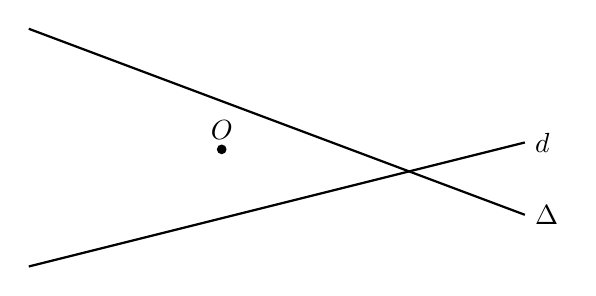
\begin{tikzpicture}[scale=0.7]
  \draw[thick] (-0.5,0.875)--(8.5,3.125) node[right] {$d$};
  \draw[thick] (-0.5,5.1875)--(8.5,1.8125) node[right] {$\Delta$};
  \fill (3,3) circle (2.5pt) node[above] {$O$};
\end{tikzpicture}
\end{center}
\begin{enumerate}
  \item نفترض أن $M$ و $N$ موجودتان. ما هي مناظرة $M$ بالنسبة إلى $O$ ؟ إلى أي مستقيم تنتمي ؟
  \item ابنِ $d'$ مناظر $d$ بالنسبة إلى $O$.
  \item استنتج بناء $N$ ثم $M$.
  \item بين أن هذا البناء يحقق المطلوب.
  \item ماذا يحدث إذا كان $\Delta$ يوازي $d$ ؟
\end{enumerate}
\axsol
\begin{enumerate}[itemsep=14pt]
  \item $O$ منتصف $[MN]$ معناه $N=S_O(M)$. وبما أن $M\in d$ فإن $N=S_O(M)\in S_O(d)=d'$. إذن $N$ تنتمي إلى $d'$ وإلى $\Delta$.
  \item مناظر المستقيم يوازيه ويُعيَّن بنقطتين : نأخذ نقطتين من $d$ ونبني مناظريهما بالنسبة إلى $O$ ؛ المستقيم المار منهما هو $d'$.
  \item $N$ هي نقطة تقاطع $d'$ و $\Delta$ ؛ ثم $M$ مناظرة $N$ بالنسبة إلى $O$.
  \begin{center}
  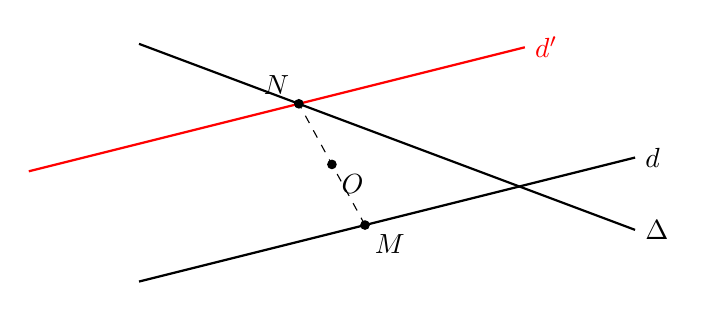
\begin{tikzpicture}[scale=0.7]
    \draw[thick] (-0.5,0.875)--(8.5,3.125) node[right] {$d$};
    \draw[thick] (-0.5,5.1875)--(8.5,1.8125) node[right] {$\Delta$};
    \draw[thick,red] (-2.5,2.875)--(6.5,5.125) node[right] {$d'$};
    \draw[dashed] (3.6,1.9)--(2.4,4.1);
    \fill (3,3) circle (2.5pt) node[below right] {$O$};
    \fill (2.4,4.1) circle (2.5pt) node[above left] {$N$};
    \fill (3.6,1.9) circle (2.5pt) node[below right] {$M$};
  \end{tikzpicture}
  \end{center}
  \item $M$ هي مناظرة $N$ بالنسبة إلى $O$ ، إذن $O$ منتصف $[MN]$. و $N\in d'=S_O(d)$ فمناظرها $M$ تنتمي إلى $S_O(d')=d$. و $N\in\Delta$ بالبناء. إذن $M\in d$ و $N\in\Delta$ و $O$ منتصف $[MN]$.
  \item إذا كان $\Delta\parallel d$ فإن $d'\parallel d$ أيضا، إذن $d'\parallel\Delta$ :
  \begin{itemize}
    \item إن كان $d'\neq\Delta$ : لا تقاطع، فلا يوجد حل.
    \item إن كان $d'=\Delta$ : أي $O$ على نفس البعد من $d$ ومن $\Delta$ ، فكل نقطة $M$ من $d$ تصلح : يوجد عدد لا نهائي من الحلول.
  \end{itemize}
  وفي حالة $\Delta$ غير موازٍ لـ $d$ (كما في الشكل) يوجد حل وحيد.
\end{enumerate}
\textbf{الفكرة :} نحوّل شرط «$O$ منتصف $[MN]$» إلى انتماء $N$ إلى مستقيم معلوم ($d'$). \quad \textbf{انتبه :} لا تنسَ مناقشة حالة التوازي.
\end{corr}

\end{document}
